% Typeset for Transactions on Architecture and Code Optimization
\documentclass[prodmode,acmtaco]{acmsmall}
\usepackage{graphicx}
\usepackage{pgfplots}
\usepackage{pgfplotstable}
\usepackage{filecontents}
\usepackage{booktabs}
\usepackage{tikz}
\usepackage{listings}
\usepackage{caption}
\usepackage{mathtools}
\usepackage{underscore}
\usepackage{url}
\usepackage{lmodern} % Much clearer text

\usetikzlibrary{patterns,shapes,positioning,calc}

\lstset{language=C, basicstyle=\ttfamily\small, columns=flexible}

\pgfplotsset{compat=1.8}

\newcommand{\perfctr}[1] {
  {\lowercase{#1}}
}

%\acmVolume{V}
%\acmNumber{N}
%\acmArticle{A}
%\acmYear{YYYY}
%\acmMonth{0}

% Page headers
\markboth{L. K. Melhus and R. E. Jensen}{Measurement Bias from Address Aliasing}

\title{Measurement Bias from Address Aliasing}
\author{
LARS KIRKHOLT MELHUS and RUNE ERLEND JENSEN
  \affil{Norwegian University of Science and Technology}}

% Motivation -- Problem statement -- Approach -- Results -- Conclusions
\begin{abstract} % Should be 150 -- 200 words max
Seemingly innocious properties of the environment, such as the contents of system environment variables, can affect the performance of computer programs.
This effect is known as \emph{measurement bias}, and has been shown to be significant, but unpredictable and difficult to deal with.

In this article we identify one of the underlying mechanics resulting in measurement bias on modern Intel microarchitectures.
Using hardware performance counters, we identify that bias is ultimately caused by \emph{address aliasing}.
When issuing load operations, the CPU is only comparing the last 12 address bits to previous stores, sometimes resulting in performance penalties from \emph{false} dependencies.

In addition to environment variable size, we show how bias can be triggered from variations in dynamically linked \emph{heap allocation} libraries.
The impact of unfavorable memory address allocations can be significant, and we demonstrate up to $2x$ speedup for a real world application.
Furthermore, the allocation pattern of common libraries such as glibc tends to give \emph{worst case} alignment by default, by favoring page alignment large allocations.
An understanding of address aliasing is necessary in order to achieve optimal performance, and we outline how to programmatically optimize for it.
\end{abstract}

% Choose from classification tree http://www.acm.org/about/class/ccs98-html
\category{C.4}{Performance of Systems}{Measurement techniques; Performance attributes}

% Terms come from a fixed list of predefined terms
\terms{Measurement, Performance}

% Free to choose keywords, but must be in alphabetical order
\keywords{4K address aliasing, heap allocators, measurement bias, memory disambiguation}

% Minimum is author, year and title
\acmformat{Lars K. Melhus and Rune E. Jensen. 2014. Measurement Bias from Address Aliasing}


\begin{document}

% Acknowledgement of support, author(s) address(es)
\begin{bottomstuff}
\end{bottomstuff}

\maketitle


\section{Introduction}
Accurately measuring the performance of computer programs is important in order to evaluate new algorithms or compare different implementations.
This process is complicated by \emph{measurment bias}, which can be a challenge for performance analysist and systems researchers.
Changes to external factors of the system, such as link ordering or the contents of environment variables, has been shown to have potentially significant impacts on performance in real applications~\cite{Mytkowicz:2009:WrongData}.
The reason this happens is because certain variables has the potential to offset memory addresses of code or data, which in turn interacts with various low level hardware buffers at runtime.
Because of the complexity of modern processors, it is often hard or even impossible to predict exactly how changes to things like system environment variables ultimately affect program execution.

To alliviate the impact of measurement bias in performance analysis, researchers have proposed to use causal analysis techniques and randomization of execution contexts~\cite{Mytkowicz:2008:OE&MB}.
Others treat the existence bias as a potential optimization problem, using search over variant spaces to find optimal environments~\cite{Knights:2009:BlindOpt}.
Our approach is analyze isolated programs in detail using \emph{performance counters}, in an attempt to identify which underlying hardware mechanisms are causing bias.

In this paper we show how some instances of measurement bias can be explained by \emph{address aliasing}, an artifact of a presumably Intel specific optimization on the out-of-order execution pipeline.
The CPU uses a heuristic for determining whether loads are dependent on previous stores, comparing only the last 12 virtual address bits.
False dependencies can happen for aliased memory accesses, incurring performance penalties.
We look at how address aliasing can trigger bias from two external factors; size of system environment variables and configuration of dynamic heap allocation libraries.

Our results show that the cost of aliasing can be significant, exemplified by a simple program with more than $2x$ speedup based in heap address alignment alone.
We also find that many heap allocation libraries tend to produce worst case behavior by default with respect to aliasing, by favoring page alignment for large allocations.
With an understanding of how false dependencies in the CPU can impact performance, measurement bias caused by it can to some extent be predicted and even accounted for in software.
We show how techniques like manual padding of allocations and dynamic detection of aliasing conditions can be used to improve performance. 
Accounting for address aliasing can give significant speedups, and our findings should motivate to exploit this in architecture-specific optimization.

The rest of this paper is structured as follows: Our methodology and experimental setup is explained in the next section.
Then section 3 introduces ``4K aliasing'', providing necessary background for interpreting the later results.
Section 4 presents an analysis of how the size of environment variables causes bias.
In Section 5 we provide a similar analysis for bias to heap address alignment.
Section 6 concludes and discusses directions for future work.



\section{Methodology}
In order to understand biased behavior it is important to be able to do precise measurements.
Besides measurement bias in itself, one must also consider \emph{observer effect}.
Any kind of instrumentation added to the code, such as a counter variable for each invocation of a function, has the potential to produce misleading results~\cite{Mytkowicz:2008:OE&MB}.
Instead, we use instrumentation provided directly by the hardware, in the form of performance counters. 
Modern processors have a set of model specific registers (MSRs) that can be configured to \emph{count} various events, such as cycles executed, branch misses, instructions fetched, and so on.
Recent Intel architectures have several hundred available events, which can give a very detailed view of what happens inside the CPU.

Performance counters are supported in the Linux kernel, and we access them via a tool called \emph{perf}. 
We use the \texttt{perf-stat} command in all experiments, which accepts raw event codes listed in the Intel reference manual \cite{Volume3B}.
A small Python script is used to collect an exhaustive set of all available counters, which amounts to about 200 on our architecture.
The same script simulates changes to environment size, which is provoked by setting a dummy environment variable to $n$ number of zero characters, starting from a minimal environment.\footnote{Because perf-stat itself adds a few variables, the environment will never be completely empty.}
Interesting events are identified by computing linear correlation to cycle count, measuring all counters over a series of execution contexts.
Cache related metrics are monitored in order to rule out cache as the underlying cause of bias, such as hit rates of micro-ops for each level of cache~\cite{OptimizationManual}.
Results are averaged over multiple runs to reduce potential random error, supplying the \texttt{-r} option to perf-stat. % Not median, good question. man perf-stat says average + std.dev. 

Because bias can be hardware dependent, and to keep the scope of this work manageable, we choose to focus on the Intel ``Haswell'' microarchitecture specifically.
Our setup consists of a 4th generation Intel\textsuperscript{\textregistered{}} Core\texttrademark{} i7-4770K processor, running 64-bit Ubuntu 14.04 LTS on kernel version 3.13.0-24-generic.
Code samples are compiled using the {\small GCC} toolchain, version 4.8.2-19ubuntu1.

We also have to ensure we are not affected by measurement bias beyond what we are actually trying to observe, and in general follow best practices on gathering data~\cite{Mytkowicz:2009:WrongData}.
Most importantly, this means keeping the memory address space under control.
For security reasons, addresses of stack, heap and dynamic libraries are often randomized at load time, a technique known as \emph{Address Space Layout Randomization}~\cite{Shackham:2004:ASLR}. % Should maybe have more generic reference
By disabling ASLR, we are able to execute the same program multiple times with identical virtual address spaces.
All benchmarks are done on a machine under minimal load, and \emph{frequency scaling} is disabled to keep the CPU's clock speed fixed.
Finally, we disable \emph{Hyper-threading}, which reduces the possibility for resource contention between threads.


\section{4K Address Aliasing}
Modern processors are \emph{superscalar}, and achieves parallelism by issuing multiple instructions simultaneously and out of order.
One of the issues that can limit throughput is dependencies between a load and previous stores.
According to Intel, typical software consists of about 38~\% memory access instructions, with about two thirds of them being loads.
To increase parallelism, modern Intel architectures use a technique called \emph{memory disambiguation} to execute memory operations out of order~\cite{Intel:2006:InsideICM:SmartMemoryAccess}. 
More often than not, loads can safely be issued before a previous store has completed and written its value to L1 cache.
Loads are therefore issued \emph{speculatively}, based on a prediction on whether it will conflict with a previous store that is still not retired.
The prediction is later verified, replaying any instructions that was wrongly assumed to have no dependencies.
Similarly, if the load and store locations are the same, the value can be \emph{forwarded} from the store before it retires.

While optimizations such as these are good on the average case, there are corner cases. 
In particular, an event known as ``4K aliasing'' can occur when the memory addresses of a store followed by a load differ by a multiple of 4096.
A store to address 0x601020 followed by a load to address 0x821020 is an aliasing pair, because the 12-bit address suffix of 0x020 is the same in both. 
Despite being independent, in these cases the memory order subsystem generates \emph{false} dependencies, and causing the load to be reissued.
The number of times this happens can be counted by the following performance counter:
\begin{description}
  \item[LD\_BLOCKS\_PARTIAL.ADDRESS\_ALIAS]
  Counts the number of loads that have partial address match with preceding stores, causing the load to be reissued.~\cite{OptimizationManual} % todo: where
\end{description}

As address aliasing depends on the memory addresses of loads and stores, environmental factors that affects memory has the potential to induce aliasing conditions.
In the following sections, we show how performance penalties from address aliasing can be the root cause of measurement bias.


\section{Bias from Environment Size}
Unless the program explicitly accesses environment variables, it is not the environment variables themselves that are important, but rather the effect their total size has on the alignment of stack.
Environment variables and program arguments are allocated in the stack section of virtual memory, before the first call frame.
Changing environment variables will therefore offset the addresses of stack, and consequently all stack allocated variables.

% Generic intro to memory layout (with focus on stack/env interaction)
Figure \ref{fig:virtualmemory} shows the relative positions of some important sections of memory at runtime, assuming a 64-bit process mapped to virtual memory. 
The stack is normally placed close to the upper address 0x7fff'ffffffff\footnote{Modern processors do not actually use the full 64-bit space, only the low order 47 bits are used for addressing memory}, but offset by environment variables.
There is still some level of stack alignment happening, independent of environment offsets. 
Normally, the stack is aligned to 16 bytes, which will be enforced by the compiler. % [ref]
Within a span of 4096 bytes there are thus 256 possible initial addresses, each representing a different execution context.
Any one of these contexts could trigger aliasing issues between stack and some other area of memory remaining unaffected by environment size.
This includes dynamic memory allocateded on heap, memory mapped files, as well as statically allocated data. 

Note that there is no clear relationship between environment size and stack location with ASLR enabled.
However, there will still be as many execution contexts with respect to aliasing (considering stack only), making any occurrences of measurement bias indeed random.
% In addition to affecting stack, ASLR also randomizes location of dynamically linked files (memory mapped), and initial position of heap.
% Moving to the lower end of the address space, we find the text, data and bss sections, which contains program code and statically allocated data.
% The memory addresses of these sections are at compile time by the linker, and can be determined by inspecting the executable.

\begin{figure}[h]
  \centering
  \caption{Organization of virtual memory for a 64-bit process.}
  \label{fig:virtualmemory}
  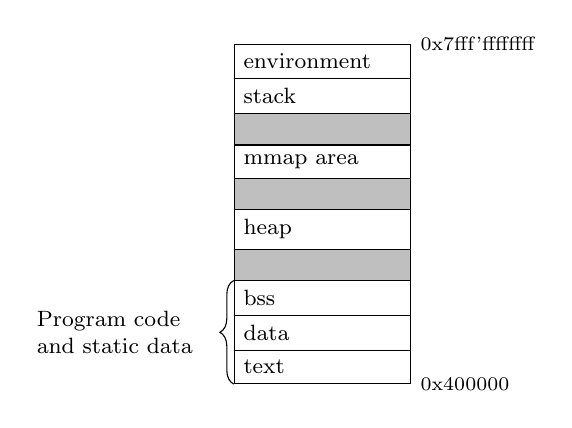
\begin{tikzpicture}[font=\footnotesize]

    % See page 453 in pgf manual
    \node [
      rectangle split, rectangle split parts=10, 
      rectangle split part fill={white, white, lightgray, white, lightgray, white, lightgray, white},
      draw, anchor=center, text width=2cm
    ] (m)
      {
        \nodepart{one}
          environment
        \nodepart{two}
          stack
        \nodepart{four}
          mmap area
        \nodepart{six}
          heap
        \nodepart{eight}
          bss
        \nodepart{nine}
          data
        \nodepart{ten}
          text
      };

    \draw [decorate, decoration={brace, amplitude=5pt}] (m.south west) -- (m.seven split west) 
      node [black, midway, xshift=-1.5cm, text width=2.0cm] 
        { Program code and static data } ;

    \node[right] at (m.north east)
      { \scriptsize{0x7fff'ffffffff} } ;

    \node[right] at (m.south east)
      { \scriptsize{0x400000} } ;

  \end{tikzpicture}
\end{figure}

% Cite does not work in acm style
% Micro-kernel presented by Mytkowicz et al~\cite{Mytkowicz:2009:WrongData}, 
\begin{lstlisting}[float=h, language=C, caption={Micro-kernel succeptible to bias from variations to system environment variables.}, label={lst:loopkernel}, frame=lines]
static int i, j, k;
int main() {
    int g = 0, inc = 1;
    for (; g < 65536; g++) {
        i += inc;
        j += inc;
        k += inc; 
    }
    return 0;
}
\end{lstlisting}

\subsection{Microkernel Analysis}
To illustrate how address aliasing can cause bias, we revisit the example first presented in ``Producing Wrong Data Without Doing Anything Obviously Wrong!'' by T. Mytkowicz et. al.~\cite{Mytkowicz:2009:WrongData}, reproduced here in Listing~\ref{lst:loopkernel}. 
This example is interesting for several reasons; the bias effects are significant and easily reproducible, while the example code is simple and straightforward to analyze.
Still, no satisfactory explanation as to what actually causes bias was given in the original paper.

% Large plot of cycle count for two 4K stack sections.
\pgfplotstableread{bin/micro-kernel-cycles.dat}{\stackoffsettable}
\begin{figure*}[t]
  \caption{Bias from environment size for micro-kernel in Listing~\ref{lst:loopkernel}. Measured average of 10 cycle count samples for 512 different environments. Spikes show aliasing case, occurring once for each 4K period}
  \label{fig:envbias}
  \begin{tikzpicture}
    \begin{axis}[
        width = \textwidth,
        height = 6cm,
        font = \footnotesize,
        xlabel=Bytes added to environment,
        ylabel=Cycles,
        domain = 0:8192,
        xtick = {0,1024,...,8192},
        xmin = 0,
        xmax = 8192,
        cycle list name = exotic
      ]
      \addplot[ycomb] table[x expr = \thisrowno{0}*16, y = cycles:u] \stackoffsettable ;
    \end{axis}
  \end{tikzpicture}
\end{figure*}

% Detailed comparison between median and worst cases.
\begin{table}[b]
  \centering
  \caption{Events with significant correlation to cycle count}
  \label{tab:loopcorrelation}
  %\renewcommand{\tabcolsep}{1pt} % Less padding between cells
  \renewcommand{\tabcolsep}{4pt} % Less padding between cells
  \pgfplotstabletypeset[
    font=\footnotesize,
    int detect, % Output whole numbers for counter values
    col sep=comma,
    columns={Performance counter, Median, [index]3, [index]4},
    column type=r,
    columns/Performance counter/.style={
      string type, 
      column type=l,
      postproc cell content/.append code={
        \pgfkeysalso{@cell content=\perfctr{##1}}
      }
    },
    every head row/.style={
      output empty row,
      before row={\toprule
        Performance counter & Median & Spike 1 & Spike 2 \\
        },
      after row=\midrule,
    },
    every last row/.style={after row=\bottomrule}
  ]{bin/micro-kernel-comparison.csv}
\end{table}

Performance counter measurements of cycle counts are shown for 512 different environment sizes in Figure~\ref{fig:envbias}.
We measure every 16 byte increment of environment size, covering two 4K periods of initial stack addresses.
A finer sampling is not necessary, because the stack is by default aligned to 16 byte.
The program is compiled with {\small{GCC}} using no optimization, as any optimization would likely disregard most of the function as redundant code, reducing it to return zero immediately.

There are clearly two worst cases, indicated by significant spikes at the 3184 and 7280 byte offsets.
We sampled an extensive set of performance counters in addition to cycle count for each execution context.
By looking at the \emph{median} value of each counter compared to the extreme cases, we narrowed down the performance events that behaved similarly to cycle count.
Table \ref{tab:loopcorrelation} shows numerical counter values for worst cases of 3184 and 7280 bytes, compared to the median over all environments.

Notice the most extreme change from median to worst case is clearly the number of alias events.
If we plot the graph for address aliasing, we see that it is near zero everywhere and spikes at exactly the points we observe bias. 
The results show a high number of resource stalls and pending memory loads when the spikes occur, which is consistent with address aliasing issues.
% Some of the other counters are less interesting; for example bus cycles, which will naturally vary with the total cycle count.
% Performance events that are obviously not indicative of any causal relationship are omitted.

On the other end we get a much lower number of reservation station (RS) stalls in the aliasing case, with a reduction from about 270,000 to about 135,000.
The reservation station buffers micro-ops for scheduling to the execution units, and a stall event means that there are no free slots available~\cite[Table 19-2]{Volume3B}.
Fewer stalls in the aliasing case could indicate less contention on the reservation station.
This probably has to do with the overall \emph{decrease} in the number of micro-ops executed per port, as all but one of the in total 8 execution ports seem to have fewer operations going in parallel.
Note that the number of micro-ops \emph{retired} overall does not change, but for some reason the micro-ops stays in the execution pipeline for a shorter time.
Our assumption is that this is a by-product of stalls generated from aliasing, causing micro-operations to be reissued.

\subsection{The Offending Variables}
Our performance counter data clearly points to address aliasing as a plausible explanation, thus the next step is to see exactly which memory accesses are aliasing. 
For that we need to know the addresses of each variable at runtime.
The program contains five variables; \texttt{g} and \texttt{inc} which are stack allocated, and \texttt{i}, \texttt{j} and \texttt{k} which are statically allocated.
Virtual memory layout of static data is decided at compile time, and we can find the location of these variables by looking at the symbol table in the ELF executable.
We find the addresses to be \texttt{\&i} = 0x60103c, \texttt{\&j} = 0x601040, and \texttt{\&k} = 0x601044.\footnote{ELF symbol tables can be read using \texttt{readelf -s}}

Observing addresses of stack allocated data at runtime is more challenging, as we have to make sure to not introduce any observer effects that alters the addresses as we are observing them.
A small amount of assembly code was added to calculate the addresses of \texttt{g} and \texttt{inc}, outputting to stdout directly using the \texttt{syscall} instruction.
Making no change to the stack allocation instructions and not affecting the addresses of static variables, the instrumented program have the exact same bias to environment size, free from observer effects.
We find that the spike in cycle count occurs precisely when the address of \texttt{inc} alias with \texttt{i}, the first spike happening when \texttt{g} is at 0x7fffffffe{\underline{038} and \texttt{inc} is at 0x7fffffffe{\underline{03c}}.
The assembly output of {\small GCC} for the inner loop is shown below, indicating the relevant load and store instructions.
There is only one store to variable \texttt{i}, which will alias with loads of \texttt{inc}.

% Refer to relevant section of the generated assembly file (in gas syntax)
\lstinputlisting[
  linerange={22-38}, 
  numbers=left,
  firstnumber=22
  ]{bin/micro-kernel-annotated.s}

Because the stack is aligned to 16 bytes, or 4 \emph{words}, there are a couple of different scenarios that could have been observed here.
Static variables are fixed and covers 12 contiguous bytes (3 words), in our case the addresses end in 0x0, 0x4 and 0xc, leaving the 0x8 slot free.
Automatic variables occupies 8 contiguous bytes on stack (2 words), in our case the addresses will always fit in the 0x8 and 0xc slots.
In this scenario, \texttt{g} will never alias with any of the static variables -- as it always covers the 0x8 slot not occupied by either of \texttt{i}, \texttt{j} or \texttt{k}.
A less fortunate scenario with respect to the number of alias events occurs when there can be collisions with both stack allocated variables, which can be achieved for example by reserving an extra 8 bytes to offset \texttt{i}, \texttt{j} into the 0x8, 0xc slots. 
While this will give significantly more alias counts, it has little effect on the total number of cycles executed.

In conclusion, we identified that address aliasing is the root cause of measurement bias from environment size for this program.
Worst case occurs for precisely one out of 256 possible initial stack addresses in every 4K segment, where resource stalls are generated because of false dependencies between stack and static data.
The program is \emph{biased} towards environment sizes that avoids this specific stack alignment.


\subsection{Avoiding Aliasing}
Addresses of automatic variables can not be determined statically, because the position of stack at runtime is generally unknown. 
In addition to being offset by environment variables, the stack address can also be perturbed by other factors such as ASLR. 
Although one can not easily know if a collision is going to happen for a given environment, it is possible to change the program to account for possible alias effects.
Shown in Listing \ref{lst:loopfixed} is a proof of concept of how alias-free code could be generated in this particular case.
If the addresses do alias, a branch to an alternative but semantically equivalent code path is performed.
Calling the function recursively will effectively allocate a new set of variables a bit further down the stack, and the alias condition is avoided.

% See analysis for results showing this does not alias
\begin{lstlisting}[float=b, language=C, caption={Dynamically detect aliasing case, and avoid by pushing another stack frame.}, label={lst:loopfixed}, frame=lines]
#define ALIAS(a, b) \
    (((long)&a) & 0xfff == ((long)&b) & 0xfff)
static int i, j, k;
int main() {
    int g = 0, inc = 1;
    if (ALIAS(inc, i) || ALIAS(g, i))
        return main();
    for (; g < 65536; g++) {
        i += inc;
        j += inc;
        k += inc;
    }
    return 0;
}
\end{lstlisting}

While this particular solution is clearly not something one would want to do in practice, it at least shows that compilers and programmers \emph{could} take measures to account for aliasing.
This becomes much more enticing when the performance penalties are more significant, which we find is often the case for aliasing heap allocations.



\section{Bias from Heap Allocation}
Address aliasing can be caused by conflicting pairs of load and store operations to any part of memory.
In the previous sections we saw collisions between static data and stack, observing bias from external conditions that affected addresses of automatic variables.
Most dynamic memory is allocated on the \emph{heap}, which is managed by an \emph{allocator}.
A heap allocator is responsible for managing dynamic memory, and ultimately assigns the actual addresses of heap allocated variables at runtime.
Heap allocation routines such as \texttt{malloc} and \texttt{free} are typically dynamically linked, for example as part of glibc, or some other library.
The particular library used therefore constitutes an important part of the execution context, as linking to a different library, or a library with some alternative configuration, can impact heap addresses at runtime.


\subsection{\texttt{malloc} will Alias by Default}
Acquiring dynamic memory at runtime is usually done by calling \texttt{malloc}, which takes a number of bytes to allocate as input, and returns a pointer to that area.
A typical malloc implementation uses different strategies for how to allocate memory depending on the \emph{size} of the request.
\begin{itemize}
  \item The ``regular'' heap area in virtual memory is used for smaller allocations. 
  Programs are initially given a relatively small heap, which the allocator can increase by calling \texttt{brk} or \texttt{sbrk} system calls.

  \item For larger allocations, it can be more efficient to use anonymous memory mapping by calling the Posix function \texttt{mmap} instead of growing the regular heap.
  One drawback of this is that it requires the memory to be zero initialized, and whether memory mapping is used or not is based on some cost heuristic employed by the allocator.
\end{itemize}
The heap section starts at a relatively low address (close to the data section), growing upwards.
Memory mapped chunks are placed towards the upper end of the virtual address space, closer to the stack.
Whether a memory allocation request is served by the heap or by memory mapping is therefore easy to determine just by looking at the actual pointer values returned.
While addresses in the regular heap can look something like 0x16e30a0 or 0x1723020, pointers returned by \texttt{mmap} are numerically much larger -- for example 0x7f0318a8f010 or 0x7f03105d2010.
This distinction is of course unimportant for application developers, as everything is conceptually the same ``heap''.
However, \texttt{mmap} has an interesting property in that allocations will always be page aligned.
The page size is 4096 bytes, meaning two pointers returned by \texttt{mmap} will \emph{always} alias.\footnote{libc's version of malloc adds 16 bytes of metadata at the beginning, therefore every memory mapped address end with 0x010.}
This behavior is often the worst case for functions that operate on two or more independent buffers, as we will see in the following sections.


\subsection{Aligned Sequential Access}
Many functions operate in a ``sliding window'' fashion; reading and writing to different buffers in some loop construction.
This type of program is potentially vulnerable to 4K aliasing, where the worst case will be when the read and write pointer addresses are aliased, continuously generating false conflicts.
As an example of this, consider a naive implementation of linear correlation shown in Listing \ref{lst:conv} (for simplicity, endpoints are not handled).
The function containins lots of interleaved loads and stores, iterating over two independent memory buffers in a tight loop.
We will see that the performance of this program greatly depends on the address alignment of each buffer, favoring memory addresses that are not closely aligned on the last 12-bits.

\lstinputlisting[
  float=t, 
  language=C, 
  caption={Naive implementation of convolution. Highly sensitive to aliasing between input and output arrays.},
  label={lst:conv},
  frame=lines
]{bin/convolution-kernel.c}

% Use mmap directly instead maybe?
By using an input size of $n=2^{20}$ (4 MiB in memory for each array), glibc's heap allocator ends up always choosing \texttt{mmap} to serve requests.
By default, even with address randomization enabled, both pointers will have the same address suffix of 0x010.
To analyse performance for different addresses, we manually insert padding to offset one of the memory mapped pointers.
This is accomplished by requesting a bit more memory, and use pointer arithmetic to offset one of the arguments before calling the function.
Controlling the offset parameter, we can create environments where the inputs are some number of \texttt{sizeof(float)} bytes apart.
Allocating and managing these buffers at startup takes a non-neglegible amount of work.
The overhead can be masked by repeatedly invoking the \texttt{convolution} kernel after allocating and initializing all the inputs.
\begin{lstlisting}
    for (i = 0; i < k; ++i)
        convolution(n, input, output + offset);
\end{lstlisting}
An estimate of the actual cost of one invocation can be calculated by averaging over a number of repeated function calls, after subtracting the constant overhead of invoking it only once.

\[
t_{\text{estimate}} = \frac{t_{k} - t_{1}}{k - 1}
\]

Our results are with $k=11$, effectively using the average over 10 loop iterations to estimate the cost of a single invocation.
For every run, performance counter measurements is also averaged over 10 samples, using the repeat mechanism of perf.

\pgfplotstableread{bin/conv-default-o2.estimate.dat}{\convtabletwo}
\pgfplotstableread{bin/conv-default-o3.estimate.dat}{\convtablethree}
\begin{figure*}[t]
  \centering
  \caption{Estimated cycle- and alias counts for different offsets between input and output arrays in convolution kernel from Listing~\ref{lst:conv}. Offset 0 means equal 12-bit address suffix, which is default behavior for \texttt{mmap} allocations. Input size $n=2^{20}$.}
  \label{fig:conv-default}
  \begin{tikzpicture}
    \begin{axis}[
        title=\texttt{cc -O2},
        font=\footnotesize,
        xlabel=Relative offset in \lstinline!sizeof(float)! bytes,
        cycle list name=black white,
        width=\textwidth/1.9, % Make it fit to text width side by side
        skip coords between index={20}{32} % Limit level of detail to fit page width nicely
      ]
      \addplot table[x expr = \thisrowno{0}, y = cycles:u] \convtabletwo ;
      \addplot table[x expr = \thisrowno{0}, y = r0107:u ] \convtabletwo ;
      \addlegendentry{Cycles} ;
      \addlegendentry{Alias} ;
    \end{axis}
  \end{tikzpicture}
  \begin{tikzpicture}
    \begin{axis}[
        title=\texttt{cc -O3},
        font=\footnotesize,
        xlabel=Relative offset in \lstinline!sizeof(float)! bytes,
        cycle list name=black white,
        width=\textwidth/1.9,
        skip coords between index={20}{32}
      ]
      \addplot table[x expr = \thisrowno{0}, y = cycles:u] \convtablethree ;
      \addplot table[x expr = \thisrowno{0}, y = r0107:u ] \convtablethree ;
      \addlegendentry{Cycles} ;
      \addlegendentry{Alias} ;
    \end{axis}
  \end{tikzpicture}
\end{figure*}

% Table with detailed performance data, use estimated for O2 because it does not need as many columns (!)
\begin{table*}[t]
  \centering
  \caption{Most interesting performance counters and correlation with cycle count for optimization O2, estimated cost accounting for constant overhead.}
  \label{tab:convstats}
  \renewcommand{\tabcolsep}{4pt} % Less padding between cells
  \pgfplotstabletypeset[
    font=\footnotesize,
    int detect, % Output whole numbers for counter values
    col sep=comma,
    columns={Performance counter, Correlation, 0, 2, 4, 8},
    column type=r,
    columns/Performance counter/.style={
      string type, 
      column type=l,
      postproc cell content/.append code={
        \pgfkeysalso{@cell content=\perfctr{##1}}
      }
    },
    columns/Correlation/.style={
      fixed,
      fixed zerofill,
      precision=2
    },
    every head row/.style={
      output empty row,
      before row={\toprule
        Performance counter & $r$ & 0 & 2 & 4 & 8 \\
        },
      after row=\midrule,
    },
    every last row/.style={after row=\bottomrule}
  ]{bin/conv-default-o2.estimate.csv}
\end{table*}

Figure~\ref{fig:conv-default} illustrates how the convolution kernel behaves for increasing offsets between heap addresses (modulo 4096), clearly indicating a relationship between address aliasing events and cycles executed.
The effects are most distinct on optimization level 2 and 3, where the ratio of cycles to alias events is most significant.
Numbers on the x axis represent the amount of offset, measured in number of \texttt{sizeof(float)} bytes.
An offset of zero is the default behavior for this program when using \texttt{malloc} and moderately large inputs.
Both for optimization level 2 and 3, the default alignment is close to worst case performance.
The differences in cycles executed is significant, with about $1.7x$ speedup for O2 and as much as $2x$ speedup for O3 for increasing relative offset.
This phenomenon is only observed for address offsets close to zero, thus we only show the first 32 data points.
If extended to cover the full width of possible offsets within a 4K segment, we see that the performance is uniform everywhere else.

More detailed performance counter data is presented in Table~\ref{tab:convstats}, where we have selected a subset that seem to correlate well with the change to cycle count.
The numbers are for the level 2 optimization case, which was chosen because the behavior was less chaotic and thus more easily represented by only a few numbers.
However, the performance data looks fairly similar between the two data sets, with a couple of events that seem to stand out.
\begin{itemize}
    \item A high number of resource stalls for the default alignment, which is reduced substantially together with increasing offsets. 
    \item A high number of cycles with memory loads pending, indicating that the pipeline is stalled waiting for load operations to resolve.
    \item Changes to the number of micro-ops executed for certain ports.
    \item Offcore requests. (++) % todo!
\end{itemize}
Interestingly, it looks like small address offsets incur a massive increase in operations issued on port 0 for the O2 case. 
On Haswell, this port handles various ALU operations, and branching together with port 6.~\cite[Figure 2.1]{OptimizationManual}
As there is also variations in the number of branch instructions executed, it seems like these counters together show that certain branch micro-ops are being re-issued.

It is also worth noticing that most cache related metrics does \emph{not} stand out in this experiment.
The L1 hit rate remains stable across all offsets, and only a neglible number of memory loads actually misses L1.

Overall it seems reasonable to conclude that the resource stalling is causing delayed execution, ultimately generated by false dependencies from address aliasing.
Variations in execution port activity, and in this case increased number of branches executed, is consistent with micro-ops being reissued after the potential conflict is detected.

We do not attempt to pinpoint exactly which assembly instructions might alias, but on a high level we can assume that the processor thinks memory accesses to \texttt{input[i]} potentially conflicts with \texttt{output[i]}.
By manually adjusting the address alignment of one of these buffers, cycle count can be reduced by as much as 50\%.
This is a speedup on top of already aggressive compiler optimization.

\subsection{Behavior of other Allocators}
As with the contents of environment variables, the exact behavior of dynamic memory allocation can typically not be known ahead of time.
Heap allocation routines such as \texttt{malloc} and \texttt{free} are usually dynamically linked and resolved at runtime, which again represents a potential source of bias.
For the code examples presented earlier, the dynamic linker will resolve \texttt{malloc} to some version of glibc, which is the default on our system.
Variations between different versions of libc, or local configurations on parameters such as thresholds for when to use \texttt{mmap} over \texttt{brk}, could trigger aliasing cases.

\begin{table*}[t]
  \centering
  \caption{Addresses returned by different heap allocators when allocating pairs of equally sized buffers.}
  \label{tab:mallocompare}
  \renewcommand{\tabcolsep}{4pt} % Less padding between cells
  \pgfplotstabletypeset[
    font=\footnotesize,
    col sep=comma,
    string type,
    columns={Allocation, 64, 5120, 65536, 1048576, 4194304},
    column type=r,
    columns/Allocation/.style={
      string type, 
      column type=l
    },
    every head row/.style={
      output empty row,
      before row={\toprule
         & 64 B & 5,120 B & 65,536 B & 1,048,576 B & 4,194,304 B \\
        },
      after row=\midrule,
    },
    every odd row/.style={after row=\midrule},
    every last row/.style={after row=\bottomrule}
  ]{bin/malloc-comparison.csv}
\end{table*}

Table \ref{tab:mallocompare} illustrates some differences that can be observed by switching heap allocator\footnote{Switching allocator was done by setting the LD\_PRELOAD environment variable.}.
In addition to glibc, where the heap allocator is called \emph{ptmalloc}, we look at the following alternatives:
\begin{itemize}
  \item Thread-Caching Malloc (tcmalloc) from Google. It claims to be time- and space efficient, and reduces lock contention for multithreaded applications~\cite{TCMalloc}.
  \item jemalloc was originally developed for FreeBSD. It aims to be a scalable general purpose allocator in single or multithreaded environments~\cite{JEMalloc}.
  \item Hoard is another project that focuses extensively on improving performance for multithreaded programs~\cite{Berger:2000:Hoard}.
\end{itemize}
The addresses of two equally sized \texttt{char} buffers allocated with \texttt{malloc} are observed for different size parameters. 
We do not care about performance, only whether the actual memory addresses returned alias or not.

For smaller allocations, we see that glibc and tcmalloc uses the normal heap area -- returning numerically low addresses.
Interestingly, jemalloc and Hoard appears to never use the normal heap, but allocate to memory mapped areas even for smaller sizes.
We see one example where one allocator yields aliasing buffers while another does not.
Allocating $2 \times 5120$ bytes returns aliasing pointers for jemalloc and Hoard, but not with glibc or tcmalloc.
Given that these results are deterministic (with ASLR disabled), it is not hard to construct a program with significant bias towards one or the other allocator.

%The purpose of this is to illustrate that allocators is yet another source of bias.
Using heap allocated memory, address aliasing is an artifact of the allocator used.
With different versions or configurations of memory allocators, any performance impact from aliasing can qualify as measurement bias.

% Most malloc alternatives focuses heavily on performance in multithreaded environments.
% Heap allocation is intrinsically inefficient in that all threads share the same address space, leading to a high potential lock contention on memory accesses.


\subsection{Ways to Deal with Address Aliasing}
Measurement bias from address aliasing can be significant in real applications, with potentially large performance penalties.
However, with an understanding of the underlying mechanism that causes bias, the effects can to some extent be predicted and accounted for in software.
The most relevant scenario to consider is probably code that can hit the aliasing \texttt{mmap} scenario, where performance impact can be consistently bad over all environments.

\paragraph{Mark buffers with \texttt{restrict}}
In our convolution kernel implementation, the compiler has to account for the fact that input and output pointers might alias, or that the buffers partially overlap.
This limits the extent generated code can keep data in registers without updating the values from memory, as a write to one buffer potentially could invalidate a cached value from the other.
The C99 keyword \emph{restrict} can be used to explicitly tell the compiler that accesses through a pointer does not alias with any other, allowing for more efficient code generation with fewer memory accesses.
\begin{lstlisting}[breaklines=true]
    void conv(int n, const float * restrict input, float * restrict output);
\end{lstlisting}
With this updated function prototype, the number of alias events is reduced by about 10 million on optimization level O2 for the default alignment, with a corresponding improvement in cycle count. % File backing this in results

\paragraph{Use a special purpose allocator}
We found that heap allocators are prone to generate pairwise aliasing buffers, the worst case for functions such as the convolution example.
A potential solution could be to apply some heuristic to randomize addresses more, and in particular not always return the same 12 bit suffix for large allocations.
This goes somewhat agains conventional wisdom that more alignment is better.
The Intel optimization manual actually mentiones this in \emph{User/Source Coding Rule 8}, suggesting that special purpose allocators could be used to avoid aliasing ~\cite{OptimizationManual}.
However, to our knowledge there are no commonly used allocators that specifically tries to mitigate aliasing in heap allocated memory.

\paragraph{Manually adjust memory}
In some cases it might make sense to explicitly control the memory addresses used, for example forcing some fixed relative offset between input and output pointers.
This can be achieved by exploiting the fact the \texttt{mmap} is in fact guaranteed to be placed at a page boundary, and use that directly instead of \texttt{malloc}.
The following approach can be used to make an anonymous memory mapping with offset \texttt{d} bytes away from page alignment.
\begin{lstlisting}[breaklines=true]
    mmap(NULL, (n + d), PROT_READ | PROT_WRITE, MAP_PRIVATE | MAP_ANONYMOUS, -1, 0) + d;
\end{lstlisting}
The same pointer difference must of course by subtracted before unmapping the memory.


\section{Conclusions}
In this article we have looked at how address aliasing can affect program performance under different memory layouts, and how it can explain certain cases of measurement bias. 
The effect is caused by the way speculative and out-of-order memory operations are handled by the CPU, only considering the last 12 address bits to resolve conflicts between load and store operations.

By analyzing an example originally presented by Mytkowicz et al. \cite{Mytkowicz:2009:WrongData}, we determined that collisions between stack variables and static data resulted in aliasing for certain stack positions.
In this case, the external trigger of bias is variations in environment size, which in turn offset the virtual addresses of stack allocated variables.

In general, any change to virtual memory layout of data can potentially introduce bias effects from address aliasing. 
We present a code example with extreme sensitivity to heap address alignment, with more than 50 \% performance variation between different memory layouts.
We find that typical heap allocators return page-aligned memory by default, which is the worst case with respect to aliasing for many algorithms.
Despite recommendations from Intel, we are not aware of any allocators that specifically addresses this issue. 
We show how manual padding of variables, and alternative alias-free code paths, can be used to avoid aliasing at runtime.
This means that an understanding of 4K address aliasing is sometimes needed to achieve optimal performance. 


\section{Acknowledgements}
This work is forked from a Master's thesis project under the supervision of Anne Cathrine Elster and Rune Erlend Jensen, looking at sources of measurment bias on the Intel Ivy Bridge architecture~\cite{MasterThesis}.


\bibliographystyle{ACM-Reference-Format-Journals}
\bibliography{references}

\end{document}
